\chapter{Software design}
\label{chap:design}

\myepigraph{If it were the case that putting effort into design reduced the effectiveness of programming I would be against it.}{Martin Fowler}{DesignStaminaHypothesis}


We focused on analyzing the 125 files that form the IPC tree of the Chromium GitHub repository \footnote{\url{https://github.com/chromium/chromium/tree/master/ipc}}. Chrome processes communicate with each other via an Inter-Process Communication IPC messaging framework built into the browser. For Windows, \textit{``named pipes"} are utilized, whereas linux builds use local Unix sockets. Most of the code that implements the IPC framework is located within the \texttt{ipc/} directory in the Chrome source tree.\\ 

\noindent The following sections delve into this framework's functionalities.
\begin{sidewaysfigure}
    \centering
    \hspace*{-2.5cm}
    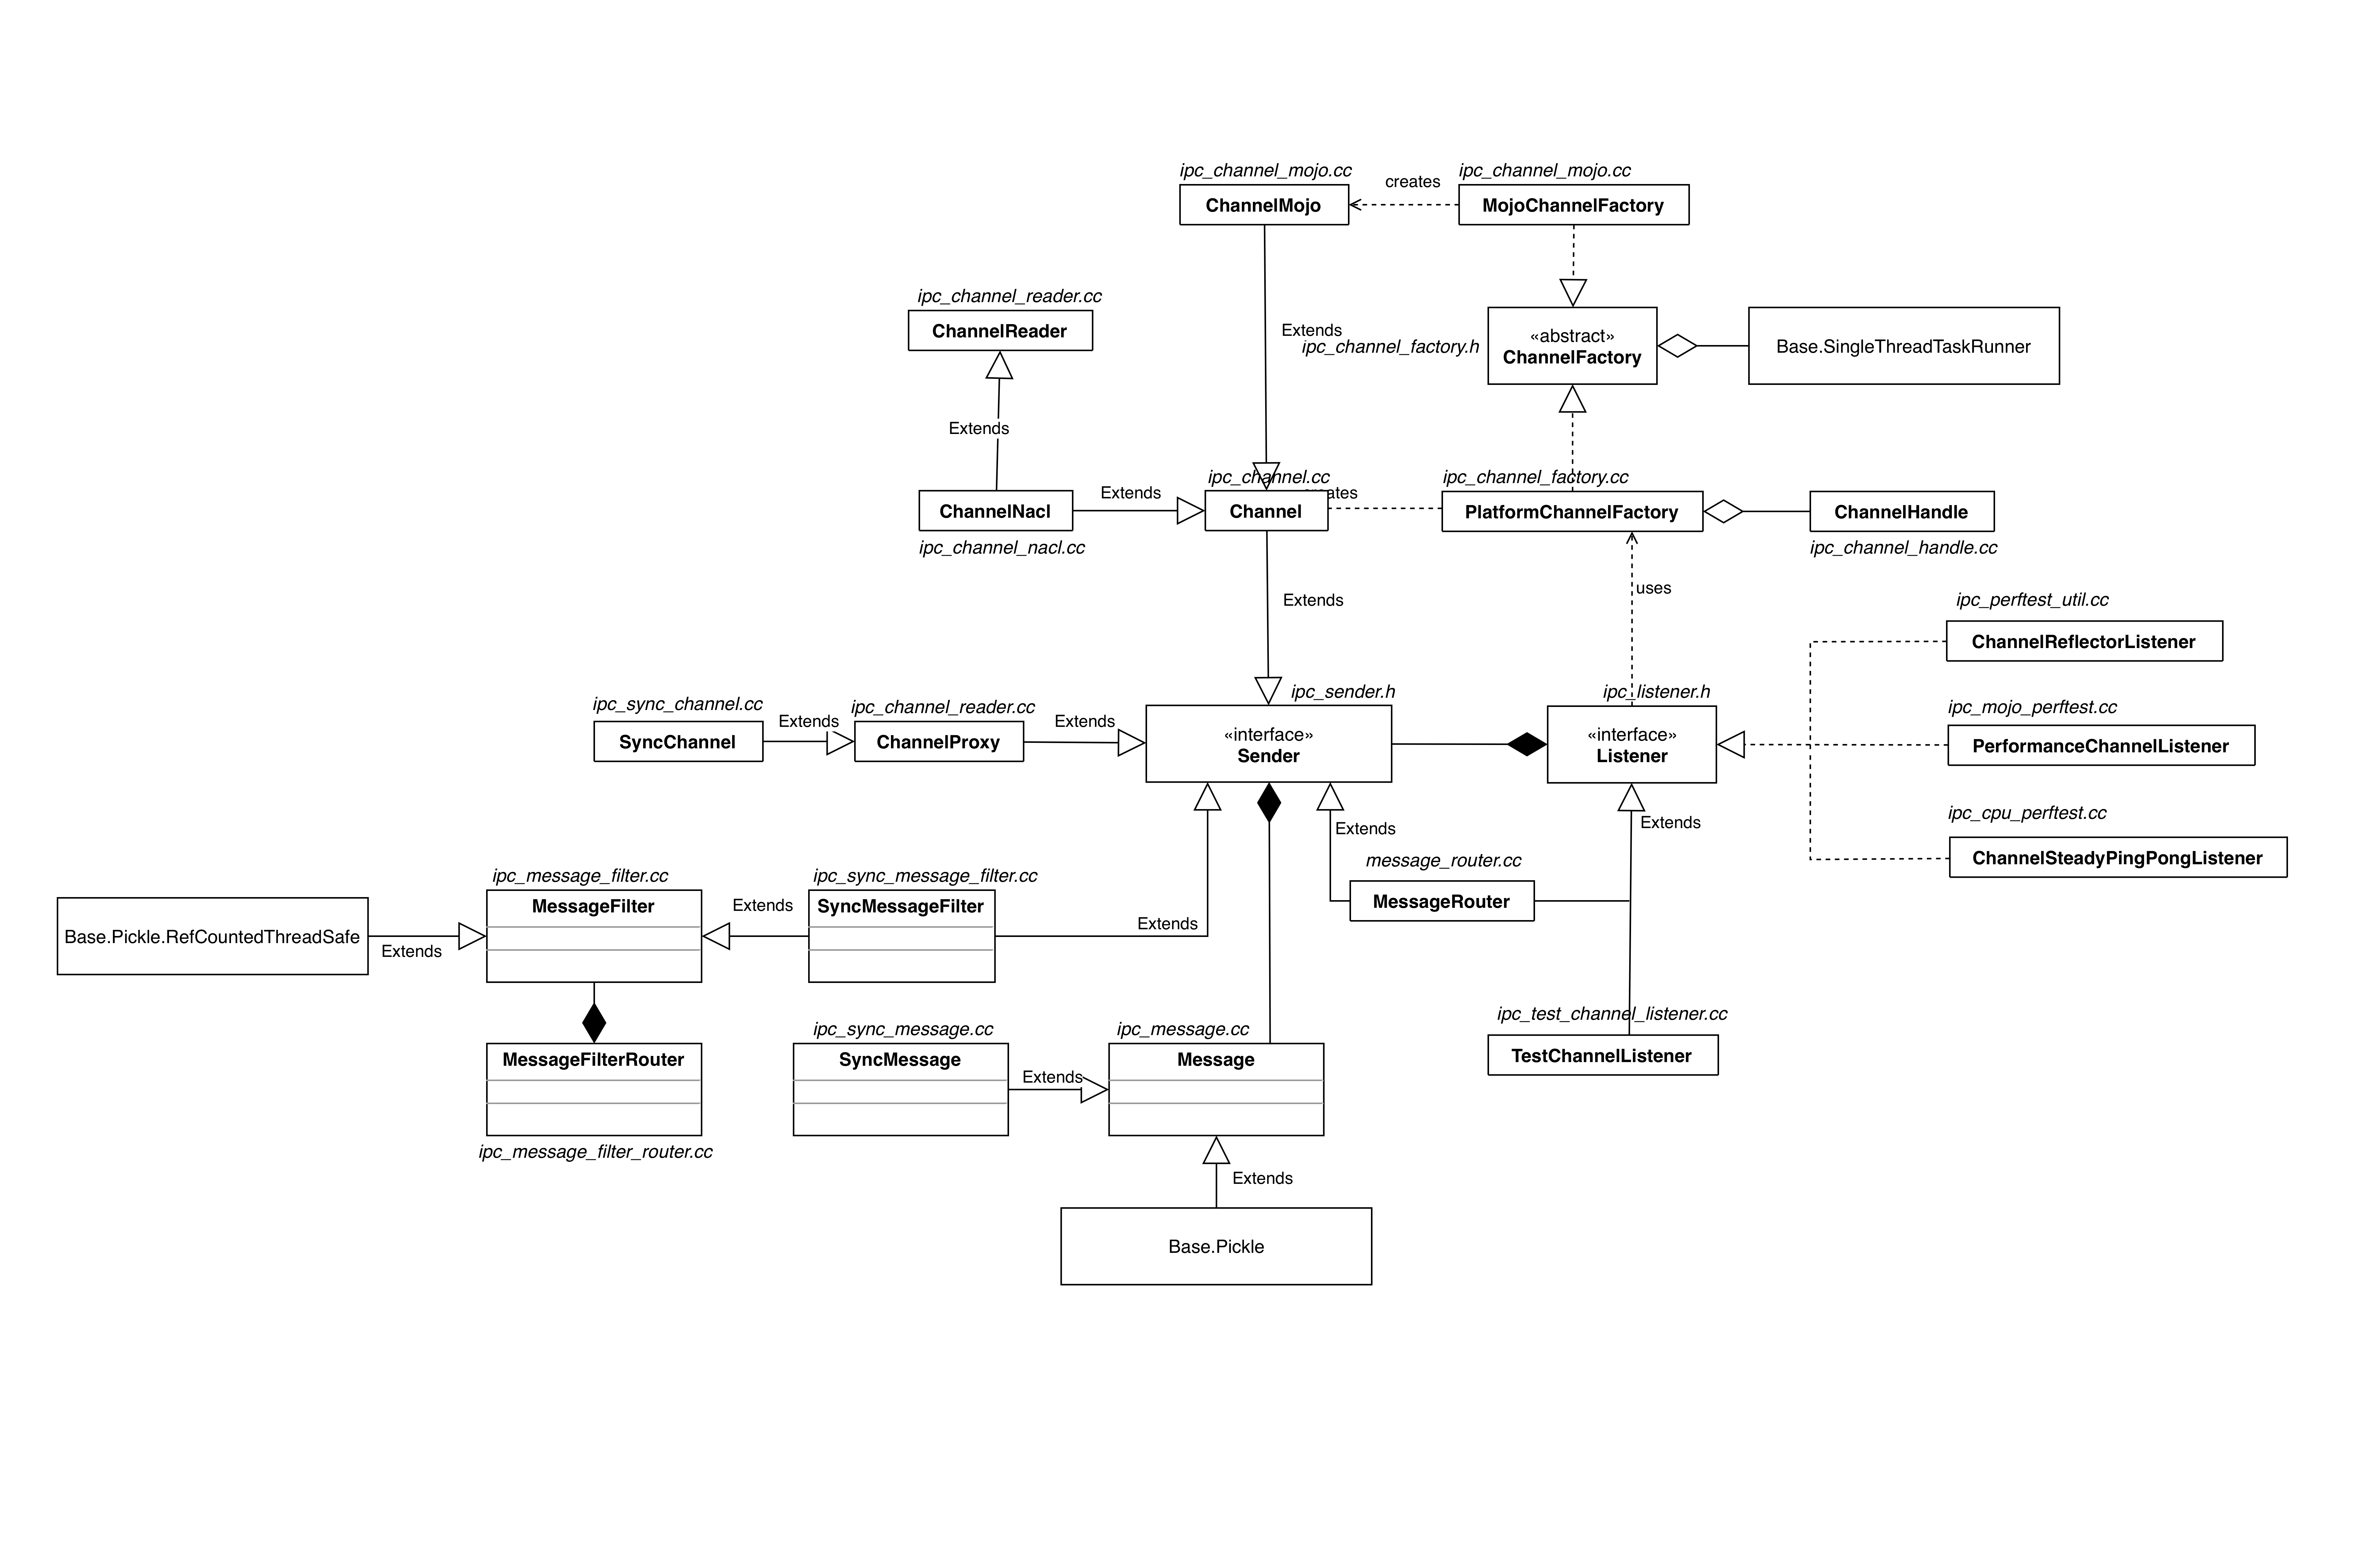
\includegraphics[width=1.2\textwidth]{img/design_min.png}
    \caption{Chromium's IPC design}
    \label{fig:design}
\end{sidewaysfigure}
\section{Channels}
The messaging framework provided by Chrome provides bidirectional communication channels between two processes through the use of a Channel object \footnote{Defined in \texttt{ipc/ipc$\_$channel.cc}}. The Channel object has one key member objects of interest to us: A listener object whose \texttt{OnMessageReceived()} function is invoked whenever a message is successfully received from the communication channel. The class definition of Listener is defined in \texttt{ipc/ipc$\_$listener.h}, but several other classes derive from it. A \texttt{Listener} object is a special object that is associated with a channel that handles incoming messages. It is used to provide the desired functionality of a given process by exposing a number of method callbacks that are invoked via the \texttt{Listener::OnMessageReceived()} function. This function typically does not handle many of the messages it receives itself; instead, it routes the messages to one of a series of objects that has been previously registered with the Listener object in question. Each of these objects registered to the listener are uniquely identified by a routing ID, and contain a series of numbered callback methods that clients may invoke. The number of the callback is unique to each object and is referred to as a message type. In the case of the browser process, the Listener object maintains a list of \texttt{MessageFilter} objects. Figure \ref{fig:design} shows the described class arrangement.


\section{Messages}

The basic unit for transmission across IPC channels is the Message object (defined in \texttt{ipc/ipc$\_$message.h}). Message objects are structured as follows:

Messages are processed in the order they are received from the communications channel by the \texttt{ChannelReader::ProcessIncomingMessage()} function \footnote{Implemented within \texttt{ipc/ipc$\_$channel$\_$reader.cc}}. Once messages have been successfully received, they are routed to an appropriate callback function through the use of a routing ID and message type, both of which are present in the Message header. The remainder of the message data is interpreted as a set of parameters for the called function, or for results of a called function in the case of reply messages.

\subsection{Types of messages}

There are two primary types of messages: ``routed" and ``control". 

\begin{description}
\item[Control] These messages are handled by the class that created the pipe. Sometimes that class will allow others to received messages by having a MessageRouter \footnote{Implemented in \texttt{ipc/message\_router.cc}} object that other listeners can register with and received ``routed" messages sent with their unique id. This is displayed in figure \ref{fig:observer}.

\item[Routed] Used to get messages to a specific RenderViewHost. 
\end{description}

\noindent Independent of the message type is whether the message is sent from:

\begin{description}
\item[Browser $\Longrightarrow$ renderer] Called Frame messages because they are being sent to the RenderFrame. 
\item[Renderer $\Longrightarrow$ browser] Called FrameHost messages because they are being sent to the RenderFrameHost.
\end{description}

\subsection{Sending messages}

Messages are sent through ``channels". In the browser, the RenderProcessHost contains the channel used to send messages from the UI thread of the browser to the renderer. Messages are sent by pointer and will be deleted by the IPC layer after they are dispatched.

\subsection{Message macros}

Special macros are used to declare messages. Messages are handled by the \texttt{IPC::Listener} interface, the most important function on which is \texttt{OnMessageReceived}. There exist a variety of macros to simplify message handling in this function.


\section{Found software Design Patterns}

In this section we'll try to extract some Design Patterns \cite{gammaetal} from the IPC Component Design Diagram in figure \ref{fig:design}.

\subsection{Adapter pattern}

The adapter design pattern is one of the twenty-three well-known GoF design patterns. It allows the interface of an existing class to be used as another interface. It is often used to make existing classes work with others without modifying their source code. 

This example (figure \ref{fig:adapter}) is is a wrapper around an OSX Mach port that can be transported across Chrome IPC channels that support attachment brokering. The send right to the Mach port will be duplicated into the destination process by the attachment broker. When used by client code in the sender process, this class is just a wrapper. The client code calls \texttt{Send(new Message(MachPortMac(mach\_port)))} and continues with its workflow. Behind the scenes, a MachPortAttachmentMac takes ownership of the Mach port. 
\begin{figure}[H]
    \centering
    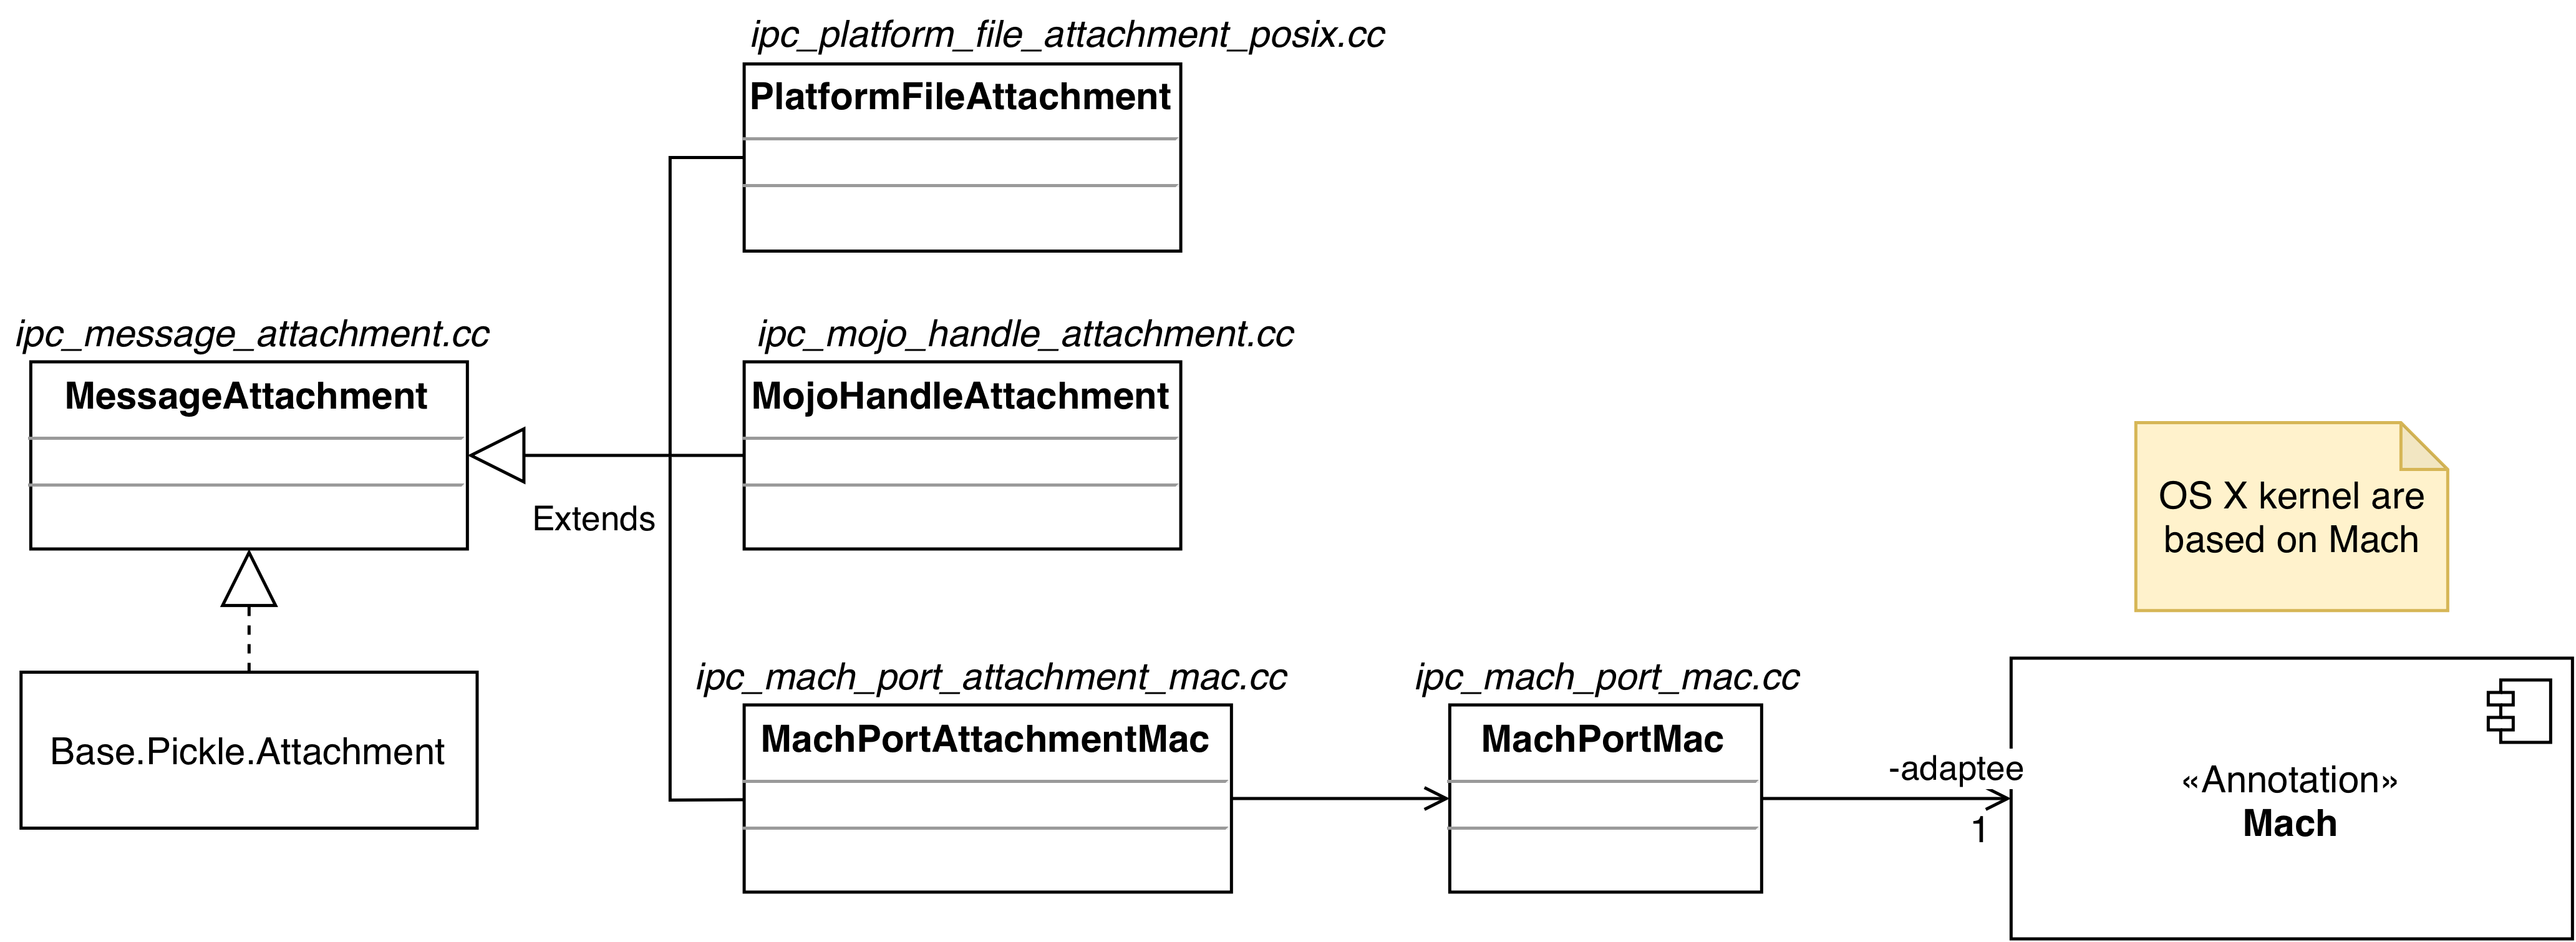
\includegraphics[width=\textwidth]{img/adapter.png}
    \caption{Adapter Pattern used to wrap OSX Mach}
    \label{fig:adapter}
\end{figure}

\subsection{Observer pattern}

\begin{sidewaysfigure}
    \centering
    {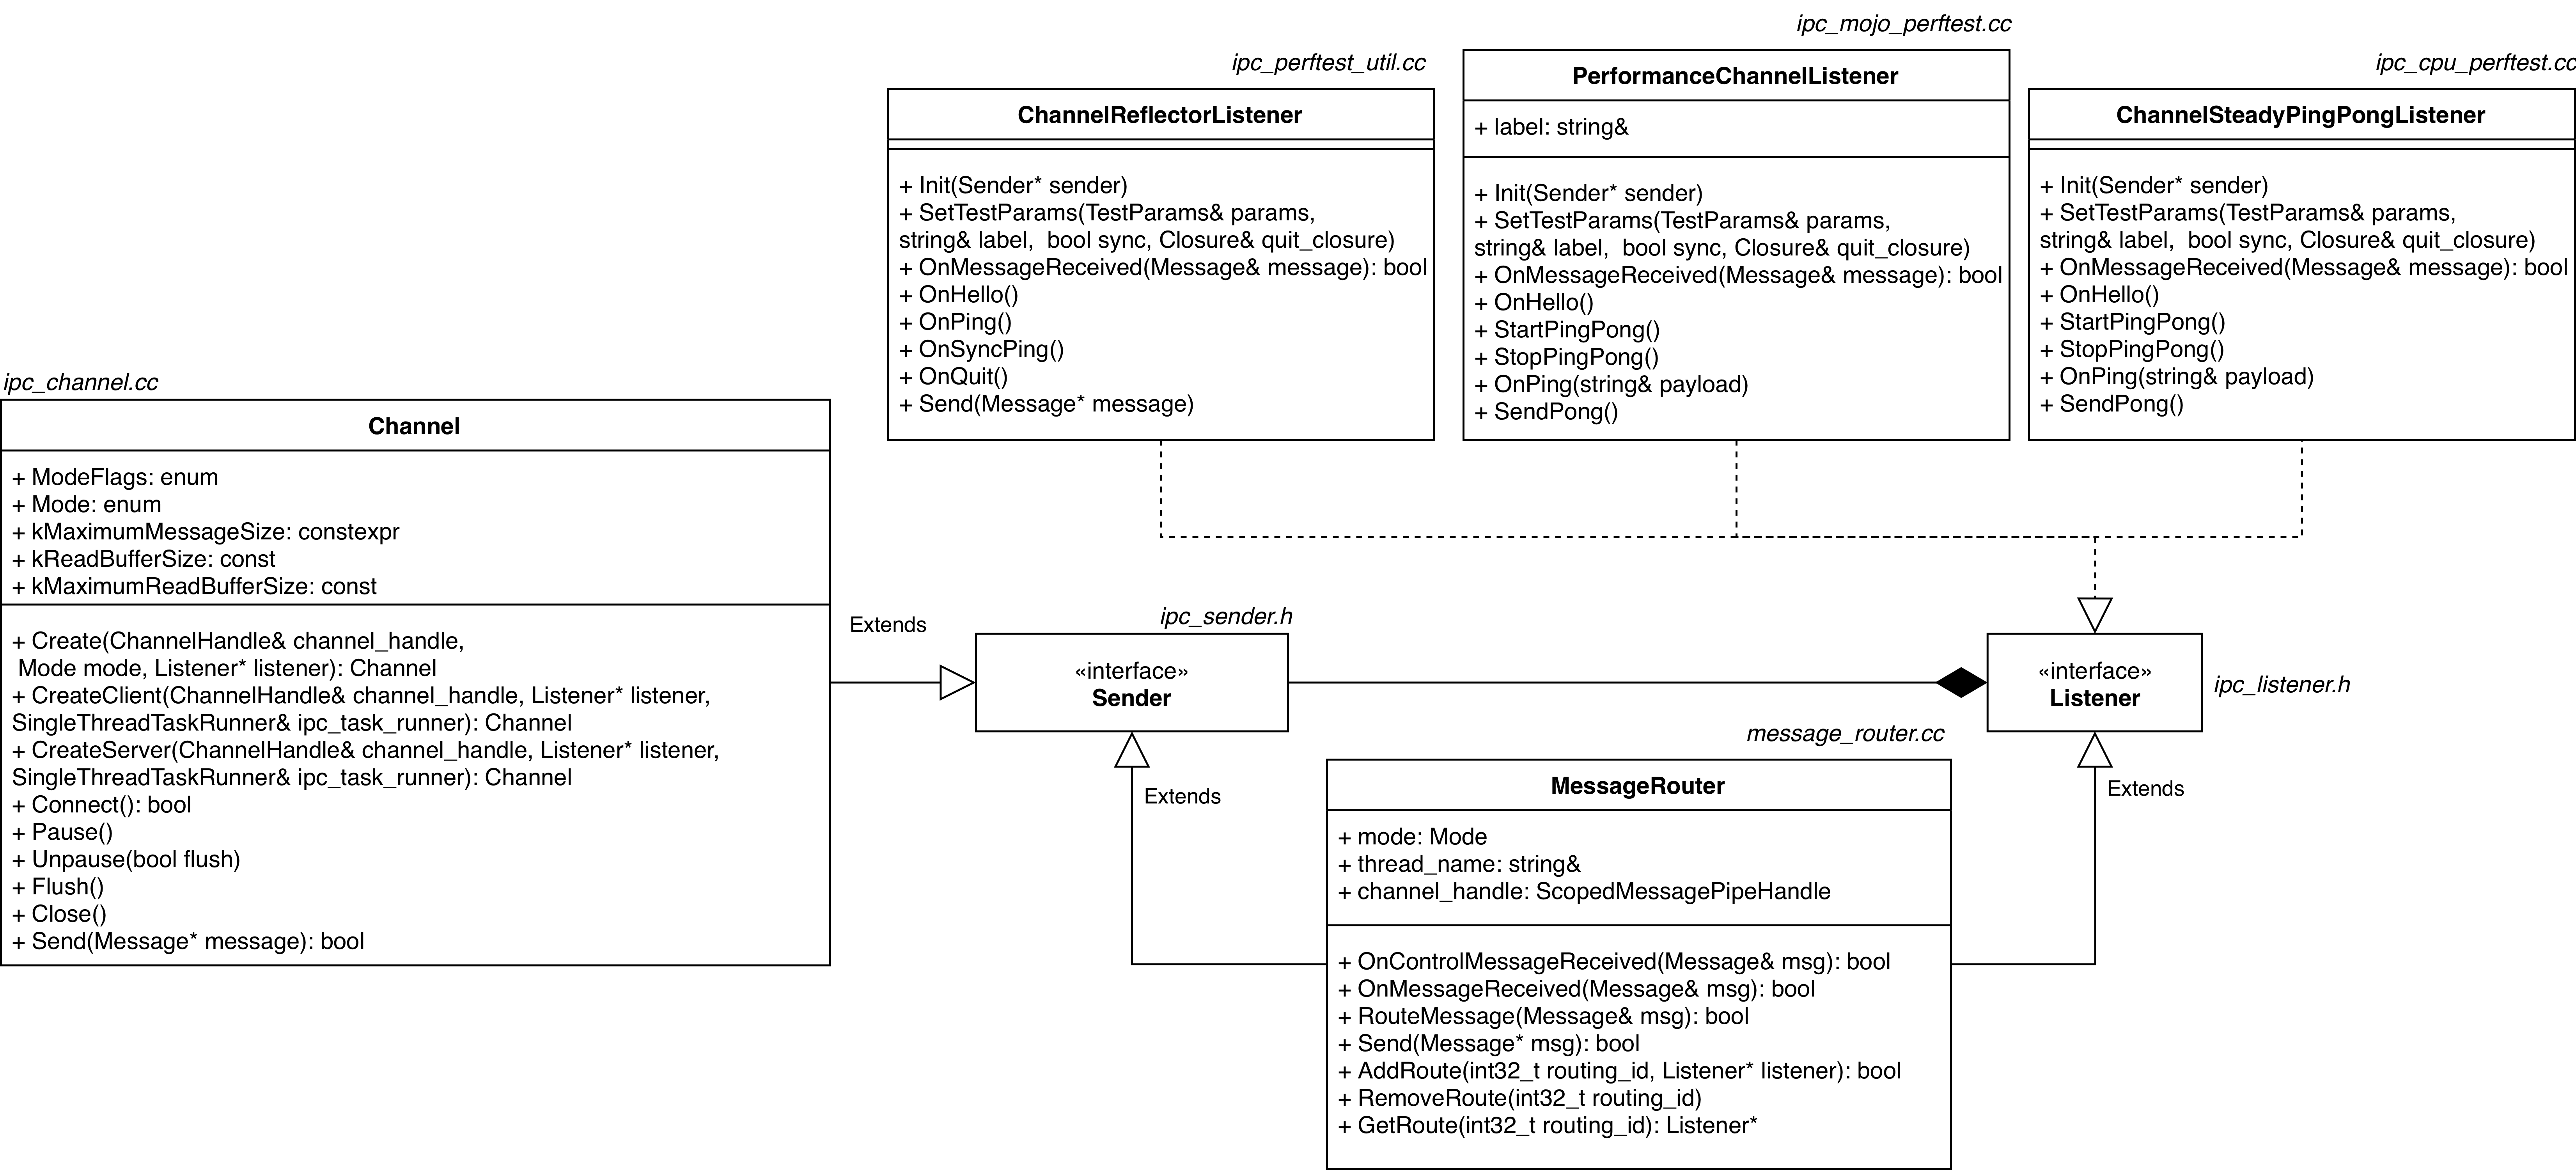
\includegraphics[width=\textwidth]{img/observer.png}}
    \caption{Observer Pattern used so listeners can register and receive messages}
    \label{fig:observer}
\end{sidewaysfigure}


In this example (figure \ref{fig:observer}), observer pattern is mainly used to implement an event handling system, where two main actor classes can be clearly identified:
\begin{description}
    \item[Subject] This component has methods to register and detach listeners to events.
    \item[Observer] Dependents. List of components to be notified upon events.
\end{description}
\begin{center}
    \begin{tabular}{p{0.5\textwidth}p{0.5\textwidth}}
    \hline
    \textbf{Problem} & \textbf{Solution} \\ \hline
    One-to-many dependency can lead to tight object coupling & Subject and Observer are loosely coupled\\ \hline
    Upon one object state change a unknown number of dependent objects must be updated & Using Subject and Observer ensures all registered observers are notified and updated\\ \hline
    one object can notify an open-ended number of other & Subject responsibility is to maintain a list of observers\\ \hline
    \end{tabular}
\end{center}

\subsection{Factory pattern}

\begin{figure}[H]
    \centering
    \makebox[\textwidth][c]{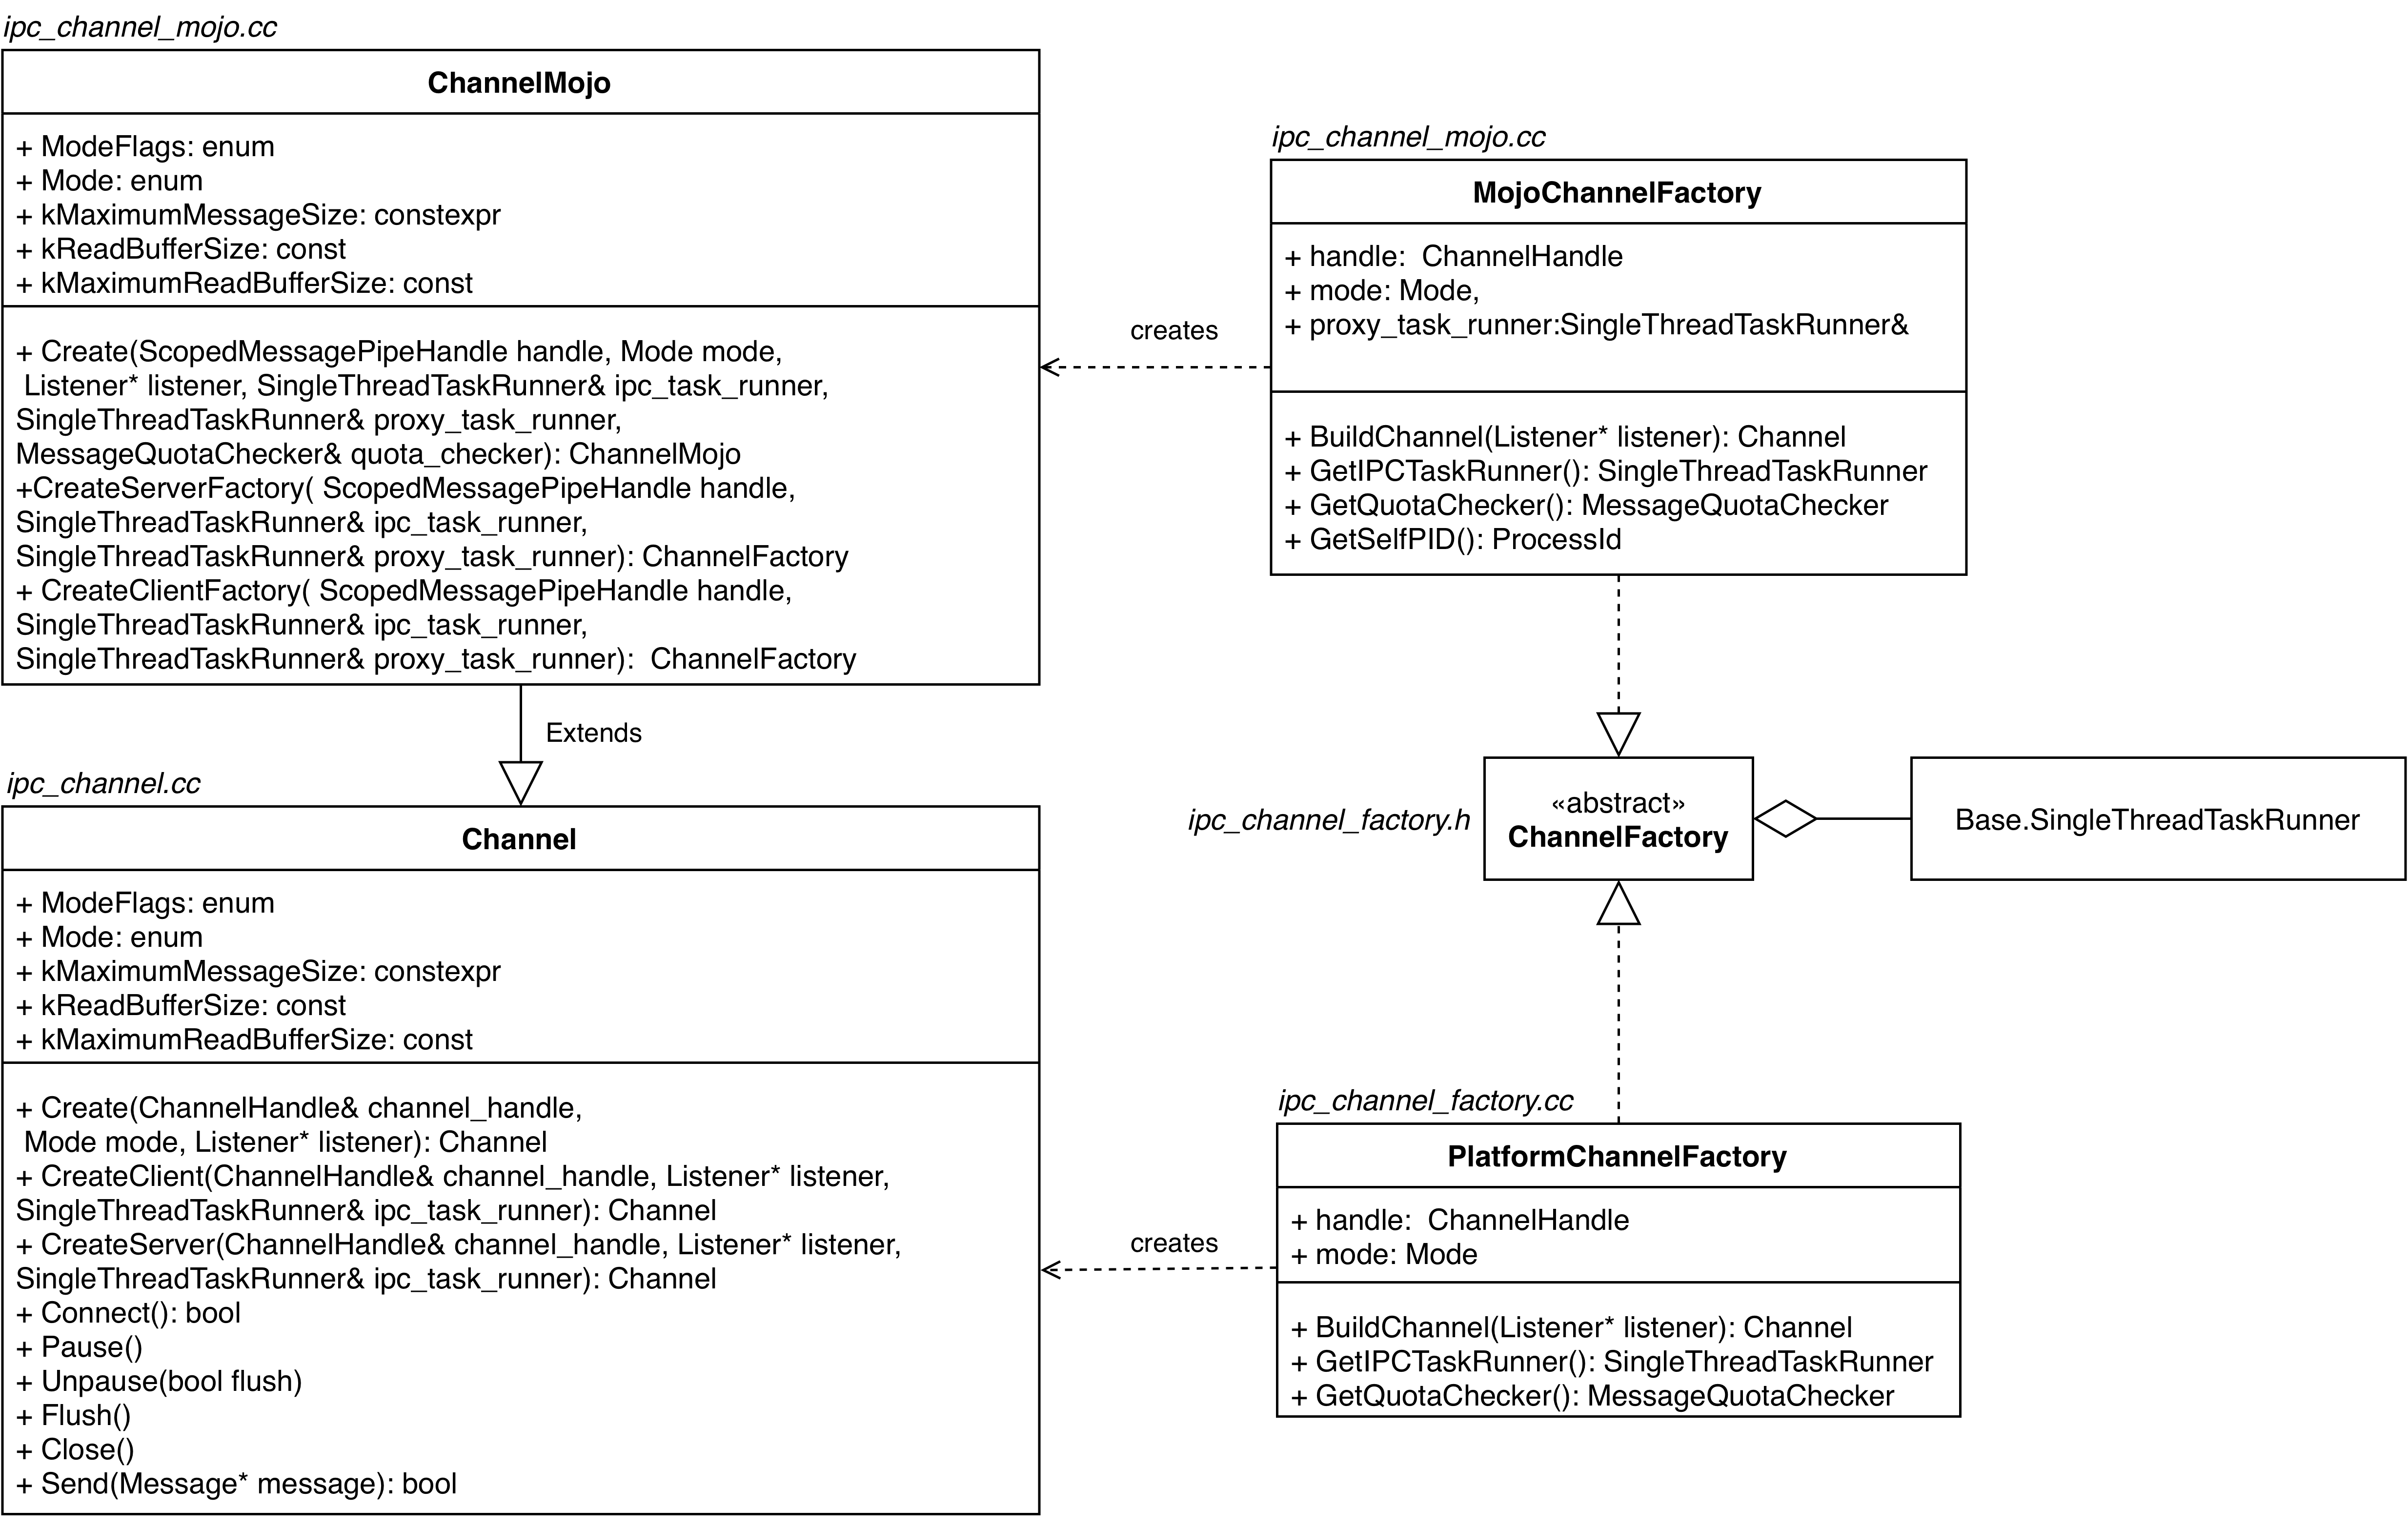
\includegraphics[width=1.2\textwidth]{img/factory.png}}
    \caption{Factory Pattern used to instantiate different channels}
    \label{fig:factory}
\end{figure}


\section{Design alternatives} 
\label{sec:bridge}

We propose the possibility using a bridge pattern to decouple several abstractions from their platform dependant implementations. 

One example can be seen in figure \ref{fig:alt}, where we found that \texttt{MojoChannelFactory's getPid} implementation depends on the platform and is currently using \texttt{ifdef} logic chains for its implementation.
\begin{sidewaysfigure}
    \centering
    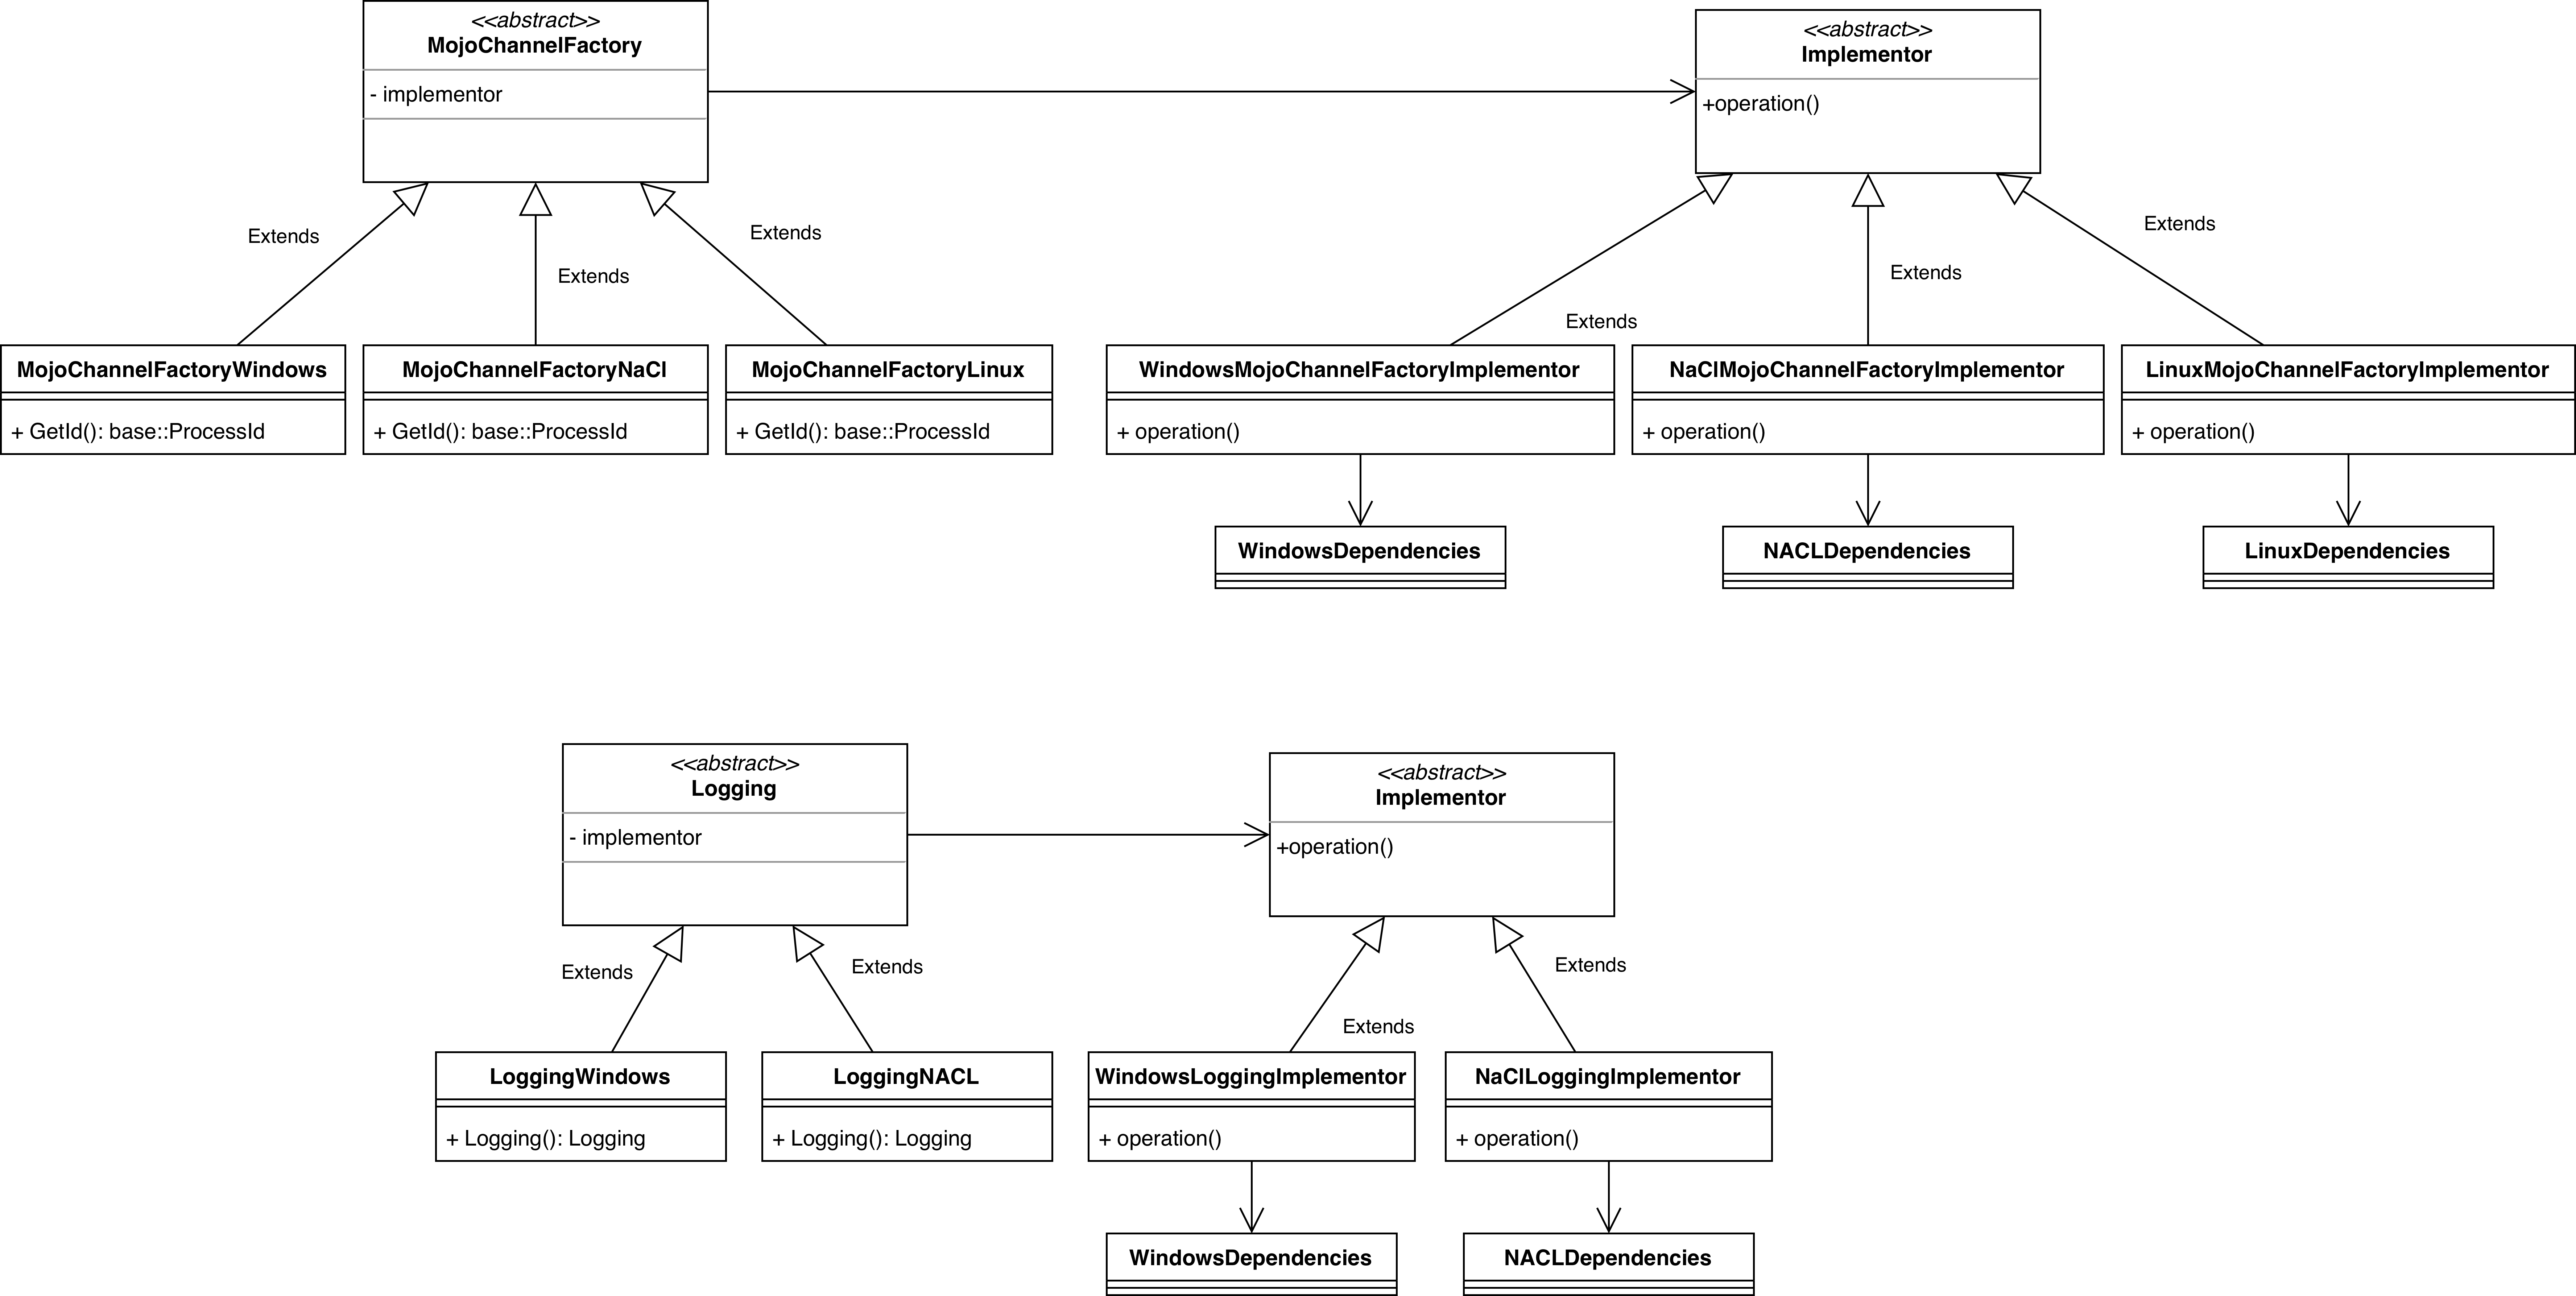
\includegraphics[width=\textwidth]{img/alt.png}
    \caption{Alternative design to decouple Logging and MojoChannelFactory abstraction from their different platform implementations}
    \label{fig:alt}
\end{sidewaysfigure}